
%----------------------------------------------------------------------------------------
\documentclass[11pt]{diazessay} % Font size (can be 10pt, 11pt or 12pt)
\usepackage{graphicx}
\usepackage{tikz}

%----------------------------------------------------------------------------------------
%	TITLE SECTION
%----------------------------------------------------------------------------------------

\title{\textbf{Proof by Minecraft} \\ {\Large\itshape The greatest proof simulator in recorded history}} % Title and subtitle

\author{\textbf{UQCS Hackathon} \\ \textit{Pajorn, Josiah, Matt, Gus, and Zwe}} % Author and institution

\date{\today} % Date, use \date{} for no date

%----------------------------------------------------------------------------------------

\begin{document}

\maketitle % Print the title section

%----------------------------------------------------------------------------------------
%	ABSTRACT AND KEYWORDS
%----------------------------------------------------------------------------------------

%\renewcommand{\abstractname}{Summary} % Uncomment to change the name of the abstract to something else

\begin{abstract}
Minecraft is widely known as a sandbox for creativity, but we extend its potential to the domain of formal reasoning: First Order Logic (FOL) and Boolean Algebra. 
Our project, Proof by Minecraft, transforms logical expressions into interactive visual proofs. 
Using Python, we parse and simplify expressions via trees and graph theory, 
then generate corresponding Minecraft circuits. 
A Tkinter-based interface allows users to input one or two expressions; the system produces a truth table, evaluates equivalence, and constructs a Minecraft representation of the logic. This approach makes formal logic both intuitive and engaging, offering a novel way to explore proofs—because sometimes, the best argument really is Proof by Minecraft.
\end{abstract}

\hspace*{3.6mm}\textit{Keywords:} First Order Logic/Boolean Algebra (FOL), Graph Theory, Trees % Keywords

\vspace{30pt} % Vertical whitespace between the abstract and first section

%----------------------------------------------------------------------------------------
%	ESSAY BODY
%----------------------------------------------------------------------------------------

\section*{Rationale - Key Ideas, Requirements, and Goals.}
The main idea behind 'Proof by Minecraft' is to make a formal logic system which is not only rigorous but visually and interactively intuitive.
It both provides a 'graphical' representation of logical expressions, and also allows users to interact with the circuit, using levers to change the value of the inputs, and to evaluate the expression.
The system also provides definitive feedback like truth tables, and equivalences which are essential for rigorously evaluating logical expressions.
By embedding First Order Logic (FOL) expressions within Minecraft, we provide users with a tangible way to explore equivalence, simplification, and proofs. Our rationale stems from three guiding goals: accessibility, interactivity, and clarity.

\subsubsection*{Key Ideas}
\begin{itemize}
    \item Each FOL expression is represented as a Minecraft world where levers act as input variables and redstone lamps display output values.  
    \item When two expressions are entered, they are rendered side by side with shared inputs, enabling direct comparison.  
    \item To evaluate equivalence, the program systematically generates all input cases ($2^n$ possibilities)* and maps them into Minecraft.
    \begin{itemize}
        \item *The reason there are $2^n$ cases is because for each event there are two possible values, true or false. So for $n$ events, there are \[
        \underbrace{2 \times 2 \times \cdots \times 2}_{n\,\mathrm{times}} = 2^n
		\]
	 combinations of truth values (since independent events are multiplied together).
	\end{itemize}
\end{itemize}

\subsubsection*{Requirements}
\begin{itemize}
    \item \textbf{Parsing and Representation:} Logical expressions must be parsed into a graph/tree structure using graph theory and algorithmic simplification.  
    \item \textbf{User Interface:} A Python GUI (Tkinter) must allow users to input expressions, following Nielsen’s 10 heuristics for usability.  
    \item \textbf{Minecraft Integration:} The parsed structure must be translated into a Minecraft world, ensuring correct placement of redstone, lamps, and levers.  
\end{itemize}

\subsubsection*{Goals}
\begin{itemize}
    \item Provide an engaging, gamified method to explore logical proofs.  
    \item Demonstrate how graph theory and algorithms can be applied creatively.  
    \item Produce both a truth table and equivalence check alongside the Minecraft visualization.  
\end{itemize}


%------------------------------------------------

\section*{Architecture and methodology}

\section{System Design}

The overall architecture of \textit{Proof by Minecraft} can be broken into four
main components: parsing, graph representation, evaluation, and Minecraft
world generation. Together these steps form a pipeline: a user enters one
or two First Order Logic (FOL) expressions, the system parses and evaluates
them, and then produces both a truth table and a Minecraft redstone circuit.

\subsubsection*{Parser}
\begin{itemize}
    \item Logical expressions are taken as strings and decomposed recursively.
    \item Operators supported include AND ($\wedge$), OR ($\vee$), and NOT ($\sim$).
    \item Bracketing ensures operator precedence is correctly maintained, with 
    special care taken for NOTs.
    \item The parser outputs a clean, bracketed form ready for tree construction.
    \item We only need AND, OR, and NOT operators, as these are sufficient to express any logical expression. (Thank you Math1081)
    \item So our system will reduce any logical expression to a form that only uses these operators, then evaluates and compares them.
    \item We used a post-order traversal to generate the final output and record important values about the nodes.
\end{itemize}

\subsubsection*{Graph Representation}
\begin{itemize}
    \item Each expression is represented as a binary tree where nodes correspond 
    to operations or variables.
    \item Internal nodes store logical operators, while leaves represent input variables.
    \item Parent/child relationships encode logical structure, enabling recursive traversal.
    \item Example: $(a \wedge b) \vee c$ becomes an OR node at the root, with an 
    AND node and variable $c$ as children.
    
\begin{center} % Centers the whole picture
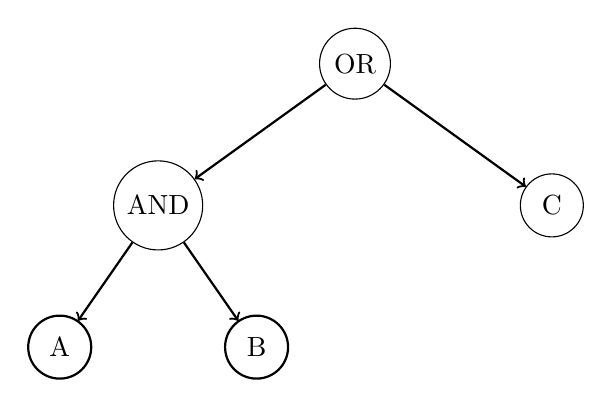
\begin{tikzpicture}[
  level distance=1.8cm,
  every node/.style={draw, circle, minimum size=8mm},
  edge from parent/.style={draw, thick, ->},
  level 1/.style={sibling distance=50mm},
  level 2/.style={sibling distance=25mm}
]
% Root
\node{OR}
  % Left subtree
  child {node {AND}
    child {node {A}}
    child {node {B}}}
  % Right child
  child {node {C}};
\end{tikzpicture}
\end{center}
	\item This tree will functionally behave the same way, but will appear slightly different to a logic gate. The way you 'read', (and our algorithm reads) this tree. Is you've decomposed the expression into two remaining parts (think of order of operations) firstly you have the LHS $(a \wedge b)$ and then the RHS $\vee c$.
	\item The following is the Logic gate representation for the aforementioned expression $(a \wedge b) \vee c$:
	\begin{figure}[h] % h = here, t = top, b = bottom
    \centering
    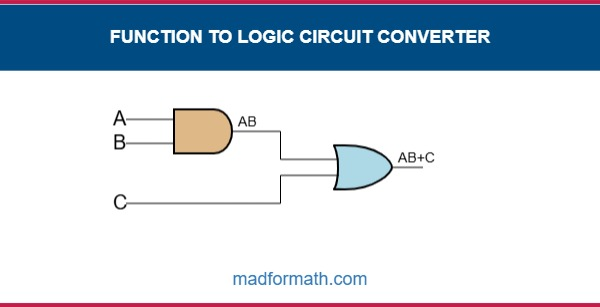
\includegraphics[width=0.75\textwidth]{LogicGate}
    \caption{Logic gate representation of the expression $(a \wedge b) \vee c$.}
    \label{fig:logic_gate}
\end{figure}

\item Compared to our tree, the logic gate representation emphasizes the flow of signals through the gates (which represent the different operators, in this case AND and OR), these operations are also expressed algebraically where AB (which is 'multiplied' and also sometimes represented as AxB, A*B, and A.B) represents $(a \wedge b)$ and A+B represents $(a \vee b)$. Whereas our tree structure highlights the hierarchical (parent/child) relationships between operations, this also makes traversal systems more effective, and easier to code - and to some - the tree diagram is more intuitive.
\medskip

\subitem *Note: Before we fleshed out the idea of Trees (a subset of graph theory), we started with a more general case of graph theory. Thinking of redstone dust as edges, and logical expressions as vertices. This was a good idea, but it was too general, and we needed to be more specific about how we were going to analyze this in Python, and translate it to minecraft. This is when we realised we could use trees.
    \begin{figure}[h]
        \centering
        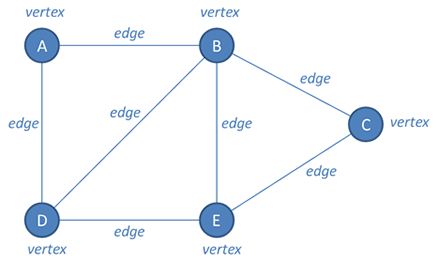
\includegraphics[width=0.6\textwidth]{gt.png}
        \caption{What a standard graph in graph theory looks like - with some examples of vertices and edges.}
        \label{fig:graph_theory_example}
    \end{figure}
\end{itemize}

\subsection*{Evaluation}
\begin{itemize}
    \item Once a tree is constructed, it can be recursively evaluated (with the method above) under any 
    assignment of truth values. 
    \item This process generates a complete truth table for the input variables.
    \item Equivalence between two expressions is determined by comparing truth 
    tables row by row. Every row of each truth table must be exactly equal for the expressions to be considered equivalent.
	\item I will show an example of this in the following section, to show you how you (and our algorithm) can evaluate the equivalence of two expressions.
\end{itemize}

\subsection{Brief Recap of Our Algorithm and how it interacts with truth tables}
\begin{itemize}
    \item \textbf{Record Output:} For each truth assignment, record the result at the root node. This forms the complete truth table for the expression.
    \item \textbf{Compare Expressions:} If two expressions are provided, generate their truth tables in the same variable order. Compare each row; if all outputs match, the expressions are equivalent.
\end{itemize}

\section*{Comparison of Two Equivalent Expressions}

We want to compare:
\[
(A \wedge B) \vee C \quad \text{and} \quad (A \vee C) \wedge (B \vee C)
\]

\bigskip

\[
\begin{array}{|c|c|c|c|c|}
\hline
A & B & C & (A \land B) \lor C & (A \lor C) \land (B \lor C) \\
\hline
0 & 0 & 0 & 0 & 0 \\
0 & 0 & 1 & 1 & 1 \\
0 & 1 & 0 & 0 & 0 \\
0 & 1 & 1 & 1 & 1 \\
1 & 0 & 0 & 0 & 0 \\
1 & 0 & 1 & 1 & 1 \\
1 & 1 & 0 & 1 & 1 \\
1 & 1 & 1 & 1 & 1 \\
\hline
\end{array}
\]

\bigskip

\begin{itemize}
    \item Since the truth tables are identical, the two expressions are equivalent.  
This shows how the algorithm evaluates different syntactic forms but produces the same output. It essentially compares these two matrices line by line, and if they are equal, then the two expressions are equivalent.
These truth tables will be produced in minecraft too, but with redstone lamps representing the truth values (on for true, off for false).
\end{itemize}

\section{Generation}

Once logical expressions are parsed, represented as trees, and evaluated,
the final step of the pipeline is \textit{generation}: producing a Minecraft
representation of the logic circuit. This process translates abstract
logical structure into tangible in-game redstone components.

\subsection{Design Challenges and Layout Considerations}

Before presenting the full solution pipeline, we summarize the principal design
difficulties encountered while mapping logical structure to a physical redstone
layout. In practice, these challenges dominated early iterations and motivated
the final heuristics we adopted.

\subsection{Physical and Geometric Constraints}

\paragraph{Redstone wiring (Manhattan geometry).}
Minecraft redstone wiring is effectively orthogonal: signals travel along block
edges (north--south, east--west) and ascend/descend in unit steps. The relevant
distance is therefore the $\ell_1$ (``taxi-cab'') metric
\[
d_1\big((x_1,z_1),(x_2,z_2)\big) \;=\; |x_1-x_2| + |z_1-z_2|,
\]
not the Euclidean metric.

\paragraph{Non-intersection of wires and 'node bloating'.}
Redstone dust cannot intersect, and adding nodes causes something I'd like to call 'node bloating', where - to prevent intersection of redstone dust - you must increase the distance between nodes, and since our NOT operation is of a different size, and it can depend on the 'parent' node as well, we needed to determine an algorithm for placement to prevent all of this.



\subsubsection*{Gate Arrangement}
\begin{itemize}
    \item Each parsed node (variable or operator) is assigned a
    2D coordinate in the Minecraft plane.
    \item Variables are aligned on the bottom row and spaced evenly.
    \item Higher-level operations are placed incrementally above their
    children, with NOT gates offset to sit directly above their operand.
    \item This ensures a clean, non-overlapping structure where
    connections can be wired in straight lines.
\end{itemize}

\subsubsection*{Redstone Placement}
\begin{itemize}
    \item Redstone wire is placed to connect the outputs of child nodes
    to their parent gate.
    \item Long runs of wire are automatically segmented with repeaters
    to prevent signal loss (e.g., every 13–15 blocks).
    \item Repeaters are oriented depending on the direction of the wire:
    upward-facing repeaters for vertical segments, and left-facing
    repeaters for horizontal runs.
\end{itemize}

\subsubsection*{Circuit Generation}
\begin{itemize}
    \item Gates (AND, OR, NOT) are summoned as invisible armor stands,
    which then trigger command block sequences to place wool, torches,
    and redstone in the correct shape.
    \item Variables are represented as floor levers, positioned below
    the circuit and aligned with their corresponding inputs.
    \item The final output of the circuit is attached to a redstone lamp,
    allowing the player to visually determine whether the expression
    evaluates to true.
\end{itemize}

\subsubsection*{Command Construction}
\begin{itemize}
    \item The entire circuit is encoded as a single Minecraft
    \texttt{/summon} command that spawns a chain of
    \texttt{falling\_block} and \texttt{command\_block\_minecart}
    entities.
    \item Each minecart contains a command to place a block (lever,
    redstone wire, repeater, lamp) at a relative coordinate.
    \item When the command is executed, the entire logical circuit
    is generated instantly in the Minecraft world.
\end{itemize}

\section*{Conclusion}

In this paper, we presented a novel approach to representing and manipulating logical expressions within the Minecraft environment. By leveraging the game's unique mechanics and our custom tools, we created a system that not only evaluates logical formulas but also visualizes them in an engaging and interactive way. 
Our implementation highlights the potential of Minecraft as a platform for educational tools, particularly in the teaching of computer science and logic. The visual and interactive nature of the system allows students to explore logical operations in a hands-on manner, transforming abstract symbols into dynamic structures that respond to user interaction.\\

\medskip
To step outside the formal language for a moment: you might reasonably ask, \textit{why?} Especially if you have examined the underlying code, and the idea can appear eccentric. The truth is that this project is as much about novelty as utility. We are passionate about both logic and Minecraft, and the intersection of these two worlds is enticing (and again, quite unique and novel). 
From a pedagogical perspective, however, the applications are very real. As a tutor myself, I frequently encounter students—particularly in Year 11 and 12 Engineering and Computer Science—who struggle to conceptualize logic gates and their behaviors. For many, the topic feels tedious and unintuitive. 
A system such as ours provides an alternative mode of engagement, allowing learners to \emph{see} and \emph{interact} (and to be honest, the best word to use here is just play.) with logical structures, rather than simply manipulating them on paper.

In this way, our work demonstrates how playful environments like Minecraft can serve as serious educational tools, making difficult concepts more accessible, intuitive, and perhaps most importantly - enjoyable.

\end{document}
